The \texttt{phaseFieldFoam}- Solver 



\begin{itemize}
    \item Moradi2021 Laplace Test
\end{itemize}


Der Solver \texttt{phaseFieldFoam} wurde bereits mehrfach für unterschiedliche Probleme validiert. Auch Simulationen mit einer Wedge wurden in \cite{holzinger2021DirectNumericalSimulation} mit Adaptiver Netzverfeinerung durchgeführt. Simulationen von Kapillaren oder auch parallelen Platten wurden in Hagg \cite{hagg2019DirekteNumerischeSimulation}, bzw. von Cai et al. \cite{cai2015NumericalSimulationWetting} durchgeführt. Samkhaniani et al. \cite{samkhaniani2021BouncingDropImpingement} simulierte einen springenden Tropfen auf einer hydrophoben Oberfläche. Viele weitere Interessante und wichtige Simulationen und Validierungen wurden mit \texttt{phaseFieldFoam} durchgeführt \cite{bodziony2023StressfulWayDroplets,yinDirectNumericalSimulation,worner2021SpreadingReboundDynamics,bagheriInterfacialRelaxationCrucial2022}, dessen einzelne Nennung den Rahmen dieser Arbeit sprengen würde. 
Da der solver bereits an vielen Stellen validiert wurde, wird in dieser Arbeit lediglich ein Laplace-Test durchgeführt. Dabei kann mit Gleichung \ref{eq: YoungLaplaceEQ} die Druckdifferenz bei einem sich einstellenden Radius des Interfaces der Simulation berechnet und mit dem Theoretischen wert Verglichen werden. Für diesen Vergleich muss der Radius des Interfaces in der Simulation bekannt sein. Um diesen zu erhalten, kann unter der Annahme, dass der Mittelpunkt des Kreises auf der Rotationsachse liegt, der Radius mit 
\begin{equation}
    r_{\mathrm{S}} = \frac{R^2}{2h}+\frac{h}{2}
\end{equation}
berechnet werden. 
\begin{figure}[h]
    \centering
    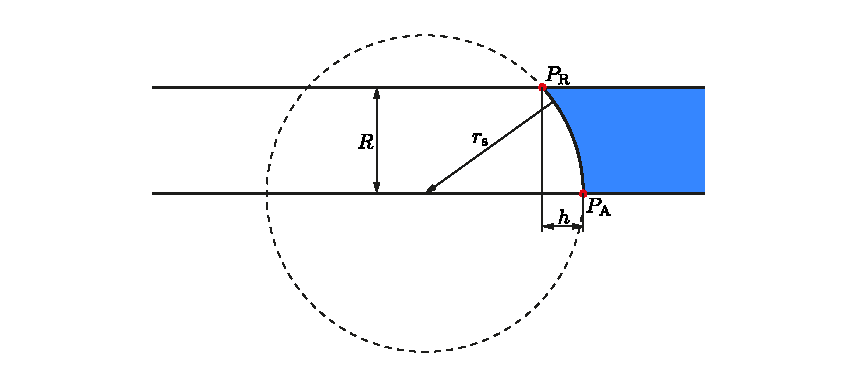
\includegraphics[width=.95\textwidth]{Pictures/RadiusCalc.pdf}
    \caption{Schematic of capillary with relevant dimension for calculation of radius}
    \label{fig: RadiusCalc}
\end{figure}

In Abbildung \ref*{fig: RadiusCalc} ist die Geometrie der Kapillare mit den relevanten Größen dargestellt. Die Punkte $P_{\mathrm{R}}$, bzw. $P_{\mathrm{A}}$ sind die Schnittpunkte des Interfaces mit der Kapillarwand und der Rotationsachse. Sind diese Punkte bekannt, kann die höhe $h$ des sphärenabschnitts berechnet werden und damit dann auch der Radius der sphäre $r_{\mathrm{S}}$ mit dem bereits bekannten Kapiilarradius $R$. Die gestrichelte Linie soll dabei verdeutlichen, dass der Radius der sphäre nicht dem der Kapillare entsprechen muss. 






